\section{Présentation}

\subsection{Préambule}
Dans le cadre de l'évaluation du projet, une défense de celui-ci a eu lieu sur base d'un document pdf 
fourni avec le projet, suivi d'une démonstration.
Ainsi, pour rendre cette dernière plus consistante, il nous a été proposé d'implémenter une autre technique relativement 
comparable à celle du LSB, appelée MSB, acronyme de Most Significant Bit.

\subsection{Most Significant Bit (M.S.B.)}
Pour coder/décoder un message, nous employons ici la technique du Most Significant Bit (MSB). \\
Cette technique consiste à se focaliser sur le bit le plus important d'un byte appelé le bit de poids fort.
Pour coder le message, il suffit de lire un byte à cacher et de l'encoder dans le bit de poids fort d'un byte choisi.
Pour décoder le message, il suffit de lire le bit de poids formats de ces bytes 'élus' et de reformer un message compréhensible.

\subsection{Encodage : extrait de code source concernant la manipulation des MSB}
\lstinputlisting[language=c, firstline=74, lastline=88]{../src/utils/bmp.c}

\newpage
\subsection{Décodage : extrait de code source concernant la manipulation des MSB}
\lstinputlisting[language=c, firstline=30, lastline=47]{../src/utils/bmp.c}
\lstinputlisting[language=c, firstline=97, lastline=100]{../src/utils/bmp.c}

\subsection{Résultats obtenus}
\begin{figure}[H]
    \centering
    \subcaptionbox{Bitmap source}{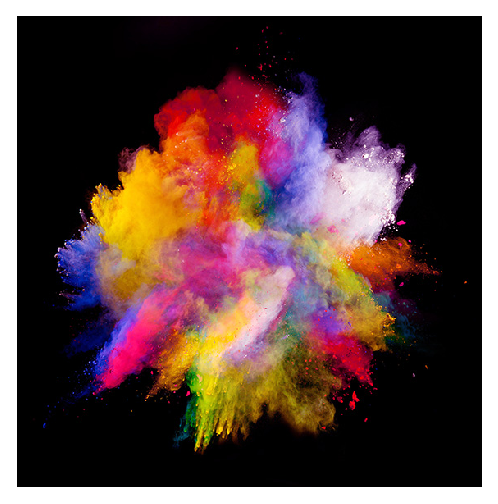
\includegraphics[width=0.45\textwidth, height=0.25\textheight]{splash_color_src.eps}}%
    \hfill
    \subcaptionbox{Bitmap dest}{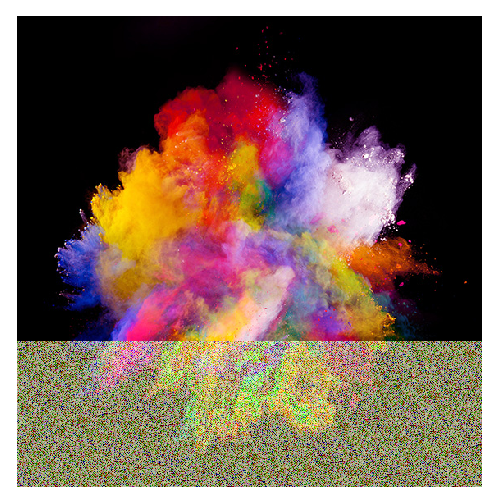
\includegraphics[width=0.45\textwidth, height=0.25\textheight]{splash_color_dest.eps}}%
    \caption{Encodage d'une vidéo .mp4 dans un bitmap}
    \caption{Altération visible du fichier d'origine}
\end{figure}
